\documentclass[11pt,a4paper]{scrartcl}
\usepackage{amssymb}
\usepackage{amsmath}
\usepackage{tikz}
\usetikzlibrary{angles,quotes,calc,intersections}
\input{"../../../../9_klase/1. Vienanariai ir daugianariai/manostilius_lt.sty"}

\title{Geometrija: Susikertantys apskritimai}
\author{Andrius Berniukevičius}

\begin{document}

\maketitle

\section{Apskritimų magija}
Sprendžiant geometrijos olimpiadinius uždavinius, vienas galingiausių įrankių yra kampų sekimas (angl. \textit{angle chasing}). Apskritimai čia atlieka ypatingą vaidmenį – jie leidžia mums akimirksniu perkelti kampus iš vienos brėžinio vietos į kitą. Pažiūrėkime, kaip šis „kampų teleportacijos“ metodas veikia praktikoje.

% ==========================================
% UŽDAVINYS IR SPRENDIMAS
% ==========================================
\vspace{0.5cm}

\begin{example}[Susikertantys apskritimai]
Du apskritimai susikerta taškuose \(P\) ir \(Q\). Per tašką \(P\) nubrėžta tiesė kerta pirmąjį apskritimą taške \(A\), o antrąjį -- taške \(B\). Per tašką \(Q\) nubrėžta kita tiesė kerta pirmąjį apskritimą taške \(C\), o antrąjį -- taške \(D\). Įrodykite, kad tiesės \(AC\) ir \(BD\) yra lygiagrečios.
\end{example}

\begin{proof}
Sprendimas:\\
Mūsų pagrindinė strategija – pasinaudoti susikertančiais apskritimais, kad „teleportuotume“ kampą prie atkarpų \(AC\) ir \(AB\) sankirtos į kitą brėžinio pusę, prie atkarpų \(BD\) ir \(AB\). Tam mums prireiks sukurti įbrėžtinius keturkampius, nubrėžiant apskritimų bendrąją stygą.

\textbf{1 žingsnis.} (Pradinis brėžinys ir tik sąlygoje duoti elementai.)
Pirmiausia nusibraižome pradinį brėžinį. Turime du susikertančius apskritimus, per susikirtimo taškus einančias tieses \(AB\) ir \(CD\), bei atkarpas \(AC\) ir \(BD\), kurių lygiagretumą bandysime įrodyti.
\begin{center}
\begin{tikzpicture}[scale=1.2]
    \coordinate (O1) at (0,0);
    \coordinate (O2) at (3,0);
    \draw[name path=C1, thick] (O1) circle (2);
    \draw[name path=C2, thick] (O2) circle (2.4);
    \path [name intersections={of=C1 and C2, by={P,Q}}];
    
    \path[name path=lineP] ($(P) + (205:5)$) -- ($(P) + (25:6)$);
    \path [name intersections={of=lineP and C1, sort by=x, by={A, P_dummy}}];
    \path [name intersections={of=lineP and C2, sort by=x, by={P_dummy2, B}}];
    
    \path[name path=lineQ] ($(Q) + (170:5)$) -- ($(Q) + (-10:6)$);
    \path [name intersections={of=lineQ and C1, sort by=x, by={C, Q_dummy}}];
    \path [name intersections={of=lineQ and C2, sort by=x, by={Q_dummy2, D}}];

    \draw[thick] (A) -- (B);
    \draw[thick] (C) -- (D);
    \draw[thick] (A) -- (C);
    \draw[thick] (B) -- (D);
    
    \foreach \p in {A,B,C,D,P,Q} \fill (\p) circle (1.5pt);
    \node[above left] at (A) {\(A\)};
    \node[above right] at (B) {\(B\)};
    \node[below left] at (C) {\(C\)};
    \node[below right] at (D) {\(D\)};
    \node[above] at (P) {\(P\)};
    \node[below] at (Q) {\(Q\)};
\end{tikzpicture}
\end{center}

\textbf{2 žingsnis.} Nubrėžiame bendrąją stygą \(PQ\) ir nagrinėjame kairįjį apskritimą.
Sujungus taškus \(P\) ir \(Q\), kairiajame apskritime susidaro įbrėžtinis keturkampis \(ACQP\). Žinome, kad įbrėžtinio keturkampio priešingų kampų suma yra \(180^\circ\), todėl \(\angle CAP + \angle CQP = 180^\circ\). Kadangi taškai \(C, Q, D\) guli vienoje tiesėje, kampai \(\angle CQP\) ir \(\angle PQD\) yra gretutiniai, todėl jų suma taip pat lygi \(180^\circ\). Iš šių dviejų faktų akivaizdu, kad išorinis keturkampio kampas prie viršūnės \(Q\) privalo būti lygus priešingam vidiniam kampui prie viršūnės \(A\):
\begin{equation*} 
\angle CAP = \angle PQD = \alpha 
\end{equation*}
Šiuos lygius kampus brėžinyje pažymime žalia spalva.
\begin{center}
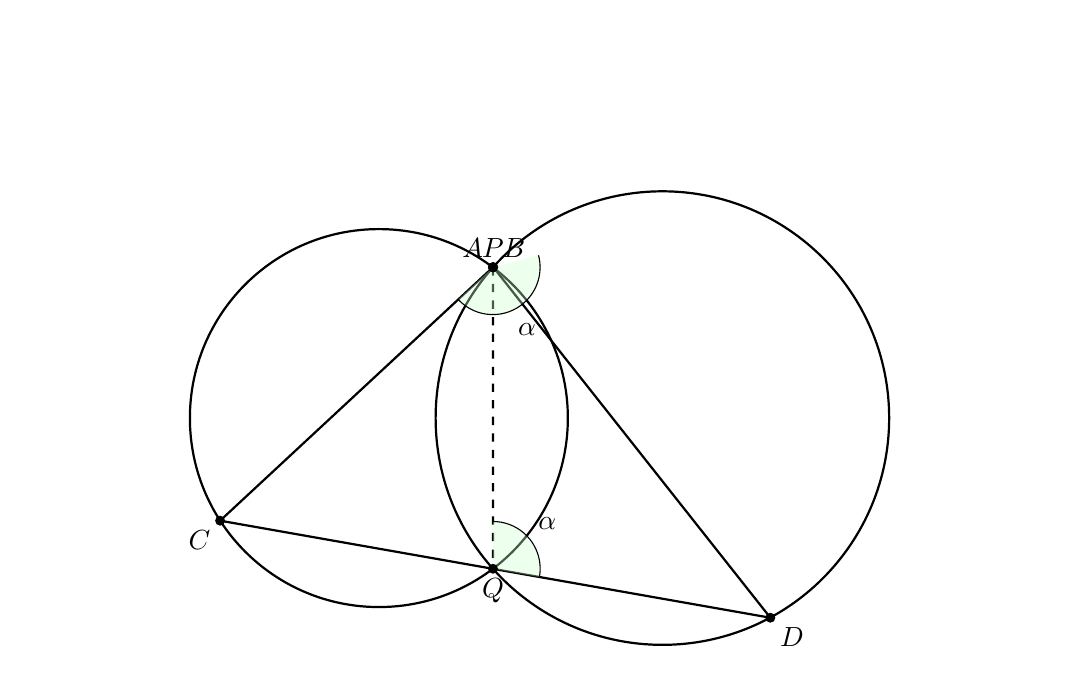
\begin{tikzpicture}[scale=1.2]
    \coordinate (O1) at (0,0); \coordinate (O2) at (3,0);
    \draw[name path=C1, thick] (O1) circle (2); \draw[name path=C2, thick] (O2) circle (2.4);
    \path [name intersections={of=C1 and C2, by={P,Q}}];
    \path[name path=lineP] ($(P) + (205:5)$) -- ($(P) + (25:6)$);
    \path [name intersections={of=lineP and C1, sort by=x, by={A, P_dummy}}];
    \path [name intersections={of=lineP and C2, sort by=x, by={P_dummy2, B}}];
    \path[name path=lineQ] ($(Q) + (170:5)$) -- ($(Q) + (-10:6)$);
    \path [name intersections={of=lineQ and C1, sort by=x, by={C, Q_dummy}}];
    \path [name intersections={of=lineQ and C2, sort by=x, by={Q_dummy2, D}}];

    \draw[thick] (A) -- (B); \draw[thick] (C) -- (D);
    \draw[thick] (A) -- (C); \draw[thick] (B) -- (D);
    
    \draw[thick, dashed] (P) -- (Q);
    
    \pic [draw, fill=green!20, fill opacity=0.35, text opacity=1, "\(\alpha\)", angle radius=6mm, angle eccentricity=1.5] {angle = C--A--P};
    \pic [draw, fill=green!20, fill opacity=0.35, text opacity=1, "\(\alpha\)", angle radius=6mm, angle eccentricity=1.5] {angle = D--Q--P};

    \foreach \p in {A,B,C,D,P,Q} \fill (\p) circle (1.5pt);
    \node[above left] at (A) {\(A\)}; \node[above right] at (B) {\(B\)};
    \node[below left] at (C) {\(C\)}; \node[below right] at (D) {\(D\)};
    \node[above] at (P) {\(P\)}; \node[below] at (Q) {\(Q\)};
\end{tikzpicture}
\end{center}

\textbf{3 žingsnis.} Kampo „teleportacija“ per dešinįjį apskritimą.
Perkeliame dėmesį į dešinįjį apskritimą. Keturkampis \(PQDB\) yra įbrėžtinis, todėl jo priešingų kampų suma taip pat turi būti \(180^\circ\). Priešingas kampas žaliajam kampui \(\angle PQD\) yra kampas prie viršūnės \(B\):
\begin{equation*} 
\angle PBD = 180^\circ - \angle PQD = 180^\circ - \alpha 
\end{equation*}
Šį naują, su pirmaisiais nesutampantį kampą, brėžinyje išskiriame raudona spalva.
\begin{center}
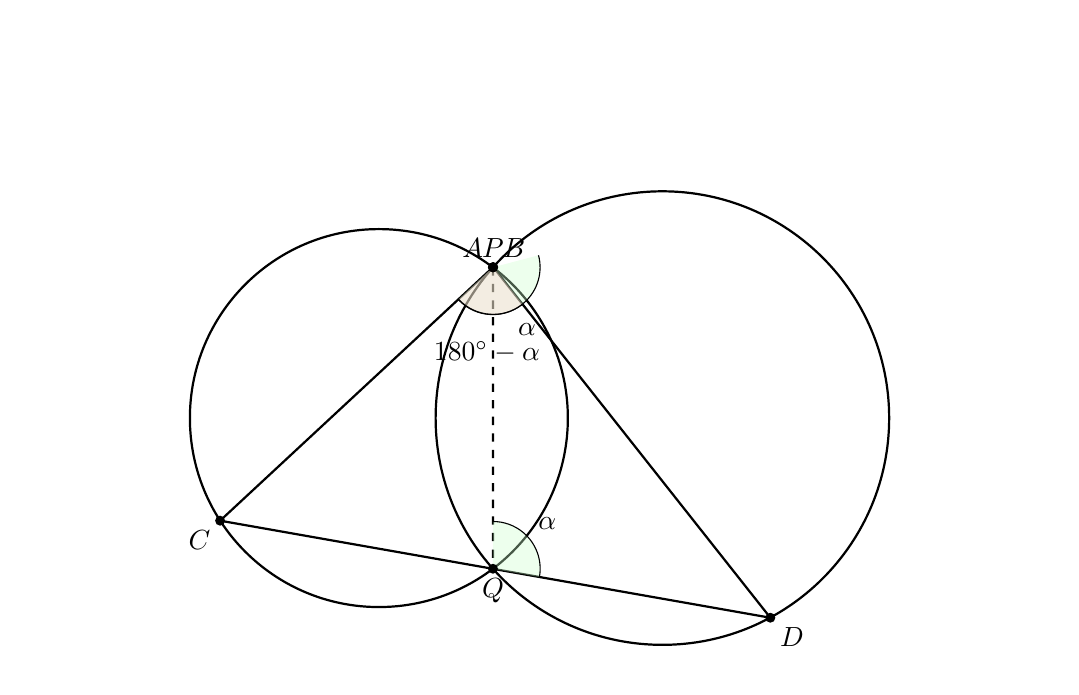
\begin{tikzpicture}[scale=1.2]
    \coordinate (O1) at (0,0); \coordinate (O2) at (3,0);
    \draw[name path=C1, thick] (O1) circle (2); \draw[name path=C2, thick] (O2) circle (2.4);
    \path [name intersections={of=C1 and C2, by={P,Q}}];
    \path[name path=lineP] ($(P) + (205:5)$) -- ($(P) + (25:6)$);
    \path [name intersections={of=lineP and C1, sort by=x, by={A, P_dummy}}];
    \path [name intersections={of=lineP and C2, sort by=x, by={P_dummy2, B}}];
    \path[name path=lineQ] ($(Q) + (170:5)$) -- ($(Q) + (-10:6)$);
    \path [name intersections={of=lineQ and C1, sort by=x, by={C, Q_dummy}}];
    \path [name intersections={of=lineQ and C2, sort by=x, by={Q_dummy2, D}}];

    \draw[thick] (A) -- (B); \draw[thick] (C) -- (D);
    \draw[thick] (A) -- (C); \draw[thick] (B) -- (D);
    \draw[thick, dashed] (P) -- (Q);
    
    \pic [draw, fill=green!20, fill opacity=0.35, text opacity=1, "\(\alpha\)", angle radius=6mm, angle eccentricity=1.5] {angle = C--A--P};
    \pic [draw, fill=green!20, fill opacity=0.35, text opacity=1, "\(\alpha\)", angle radius=6mm, angle eccentricity=1.5] {angle = D--Q--P};
    \pic [draw, fill=red!20, fill opacity=0.35, text opacity=1, "\(180^\circ-\alpha\)", angle radius=6mm, angle eccentricity=1.8] {angle = P--B--D};

    \foreach \p in {A,B,C,D,P,Q} \fill (\p) circle (1.5pt);
    \node[above left] at (A) {\(A\)}; \node[above right] at (B) {\(B\)};
    \node[below left] at (C) {\(C\)}; \node[below right] at (D) {\(D\)};
    \node[above] at (P) {\(P\)}; \node[below] at (Q) {\(Q\)};
\end{tikzpicture}
\end{center}

\textbf{4 žingsnis.} Lygiagretumo nustatymas remiantis vienašalių kampų suma.
Prisiminkime pradinį tikslą – įrodyti, kad tiesės \(AC\) ir \(BD\) yra lygiagrečios. Jas abi kerta tiesioji \(AB\), sudarydama vienašalius kampus prie viršūnių \(A\) ir \(B\). Apskaičiuokime jų sumą:
\begin{equation*} 
\angle CAB + \angle ABD = \alpha + (180^\circ - \alpha) = 180^\circ 
\end{equation*}
Geometrijoje gerai žinoma taisyklė: jei tiesei kertant dvi kitas tieses vienašalių kampų suma lygi lygiai \(180^\circ\), tai tos dvi kirstosios tiesės privalo būti lygiagrečios. Kadangi būtent tai ir gavome, atsakymas garantuotas.
\begin{center}
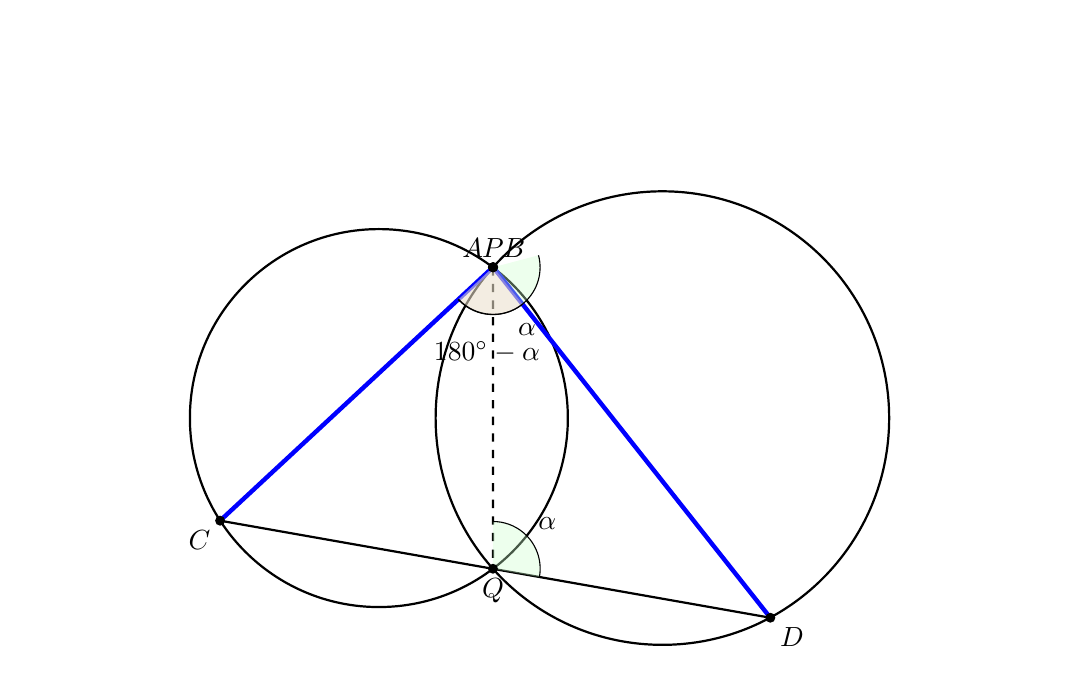
\begin{tikzpicture}[scale=1.2]
    \coordinate (O1) at (0,0); \coordinate (O2) at (3,0);
    \draw[name path=C1, thick] (O1) circle (2); \draw[name path=C2, thick] (O2) circle (2.4);
    \path [name intersections={of=C1 and C2, by={P,Q}}];
    \path[name path=lineP] ($(P) + (205:5)$) -- ($(P) + (25:6)$);
    \path [name intersections={of=lineP and C1, sort by=x, by={A, P_dummy}}];
    \path [name intersections={of=lineP and C2, sort by=x, by={P_dummy2, B}}];
    \path[name path=lineQ] ($(Q) + (170:5)$) -- ($(Q) + (-10:6)$);
    \path [name intersections={of=lineQ and C1, sort by=x, by={C, Q_dummy}}];
    \path [name intersections={of=lineQ and C2, sort by=x, by={Q_dummy2, D}}];

    \draw[thick] (A) -- (B); \draw[thick] (C) -- (D);
    \draw[ultra thick, blue] (A) -- (C); \draw[ultra thick, blue] (B) -- (D);
    \draw[thick, dashed] (P) -- (Q);
    
    \pic [draw, fill=green!20, fill opacity=0.35, text opacity=1, "\(\alpha\)", angle radius=6mm, angle eccentricity=1.5] {angle = C--A--P};
    \pic [draw, fill=green!20, fill opacity=0.35, text opacity=1, "\(\alpha\)", angle radius=6mm, angle eccentricity=1.5] {angle = D--Q--P};
    \pic [draw, fill=red!20, fill opacity=0.35, text opacity=1, "\(180^\circ-\alpha\)", angle radius=6mm, angle eccentricity=1.8] {angle = P--B--D};

    \foreach \p in {A,B,C,D,P,Q} \fill (\p) circle (1.5pt);
    \node[above left] at (A) {\(A\)}; \node[above right] at (B) {\(B\)};
    \node[below left] at (C) {\(C\)}; \node[below right] at (D) {\(D\)};
    \node[above] at (P) {\(P\)}; \node[below] at (Q) {\(Q\)};
\end{tikzpicture}
\end{center}

Įrodyta. \hfill \(\square\)
\end{proof}

\end{document}